\documentclass{article}
\usepackage[T2A]{fontenc}
\usepackage[utf8]{inputenc}
\usepackage[serbian]{babel}
\usepackage{graphicx}
\usepackage{url}
\usepackage{subcaption}


\title{Класификација филмских жанрова на основу музике из филмова}
\author{Дуња Мијачић 2019/74}
\date{\today}


\begin{document}



\maketitle

\newpage

\section{Увод}
Филмови су уметнички израз који комбинује визуелне и аудитивне компо- ненте како би пренели причу и емоције публици. Један од клучних елемената који доприноси атмосфери и емоционалном доживљају филма је музика. У овом раду истражујемо класификацију филмских жанрова на основу музике која се појављује у филмовима. Специфично, анализирамо музику из пет различитих жанрова: романтична, вестерн, мјузикл, хорор и научна фантастика. Циљ је разумети карактеристике и емоције које се преносе кроз музику у овим жанровима.

\subsection{Опис музике за различите филмске жанрове}

\begin{itemize}
\item \textbf{Романтика:} Музика за романтичне филмове често се карактерише нежним мелодијама и сложеним хармонијама. Ова врста музике преноси љубав, страст и романтични доживљај. Жичани инструменти често доминирају у оваквим композицијама.

\item \textbf{Мјузикл:} Мјузикли су познати по својим веселим и мелодичним песмама. Музика за мјузикле често интегрише песме и плес у причу филма. Ова врста музике подстиче енергију и емоционалну изражајност.

\item \textbf{Вестерн:} За вестерн филмове, музика је често инспирисана западним темама и традицијама. Употреба гитаре, хармонике и гласова најављује овај жанр. Музика је обично меланхолична и приказује тешке услове и борбу на дивљем западу.

\item \textbf{Хорор:} Музика у хорор филмовима има за циљ да изазове напетост и страх код гледалаца. Тамни и једноставни звуци, уз употребу оргуља и удараљки, стварају узбудљиву и неизвесну атмосферу. Музика често има необичне и дисторзиране звукове.

\item \textbf{Научна фантастика (Sci-Fi):} Музика за научно-фантастичне филмове често је футуристичка и електронска. Синтисајзери и компјутерски генерисани звукови доприносе приказу будућности и неизвесности. Мелодије су обично комплексне и амбијенталне.
\end{itemize}

\begin{figure}[htbp]
  \centering
  \begin{subfigure}{0.45\textwidth}
    \centering
    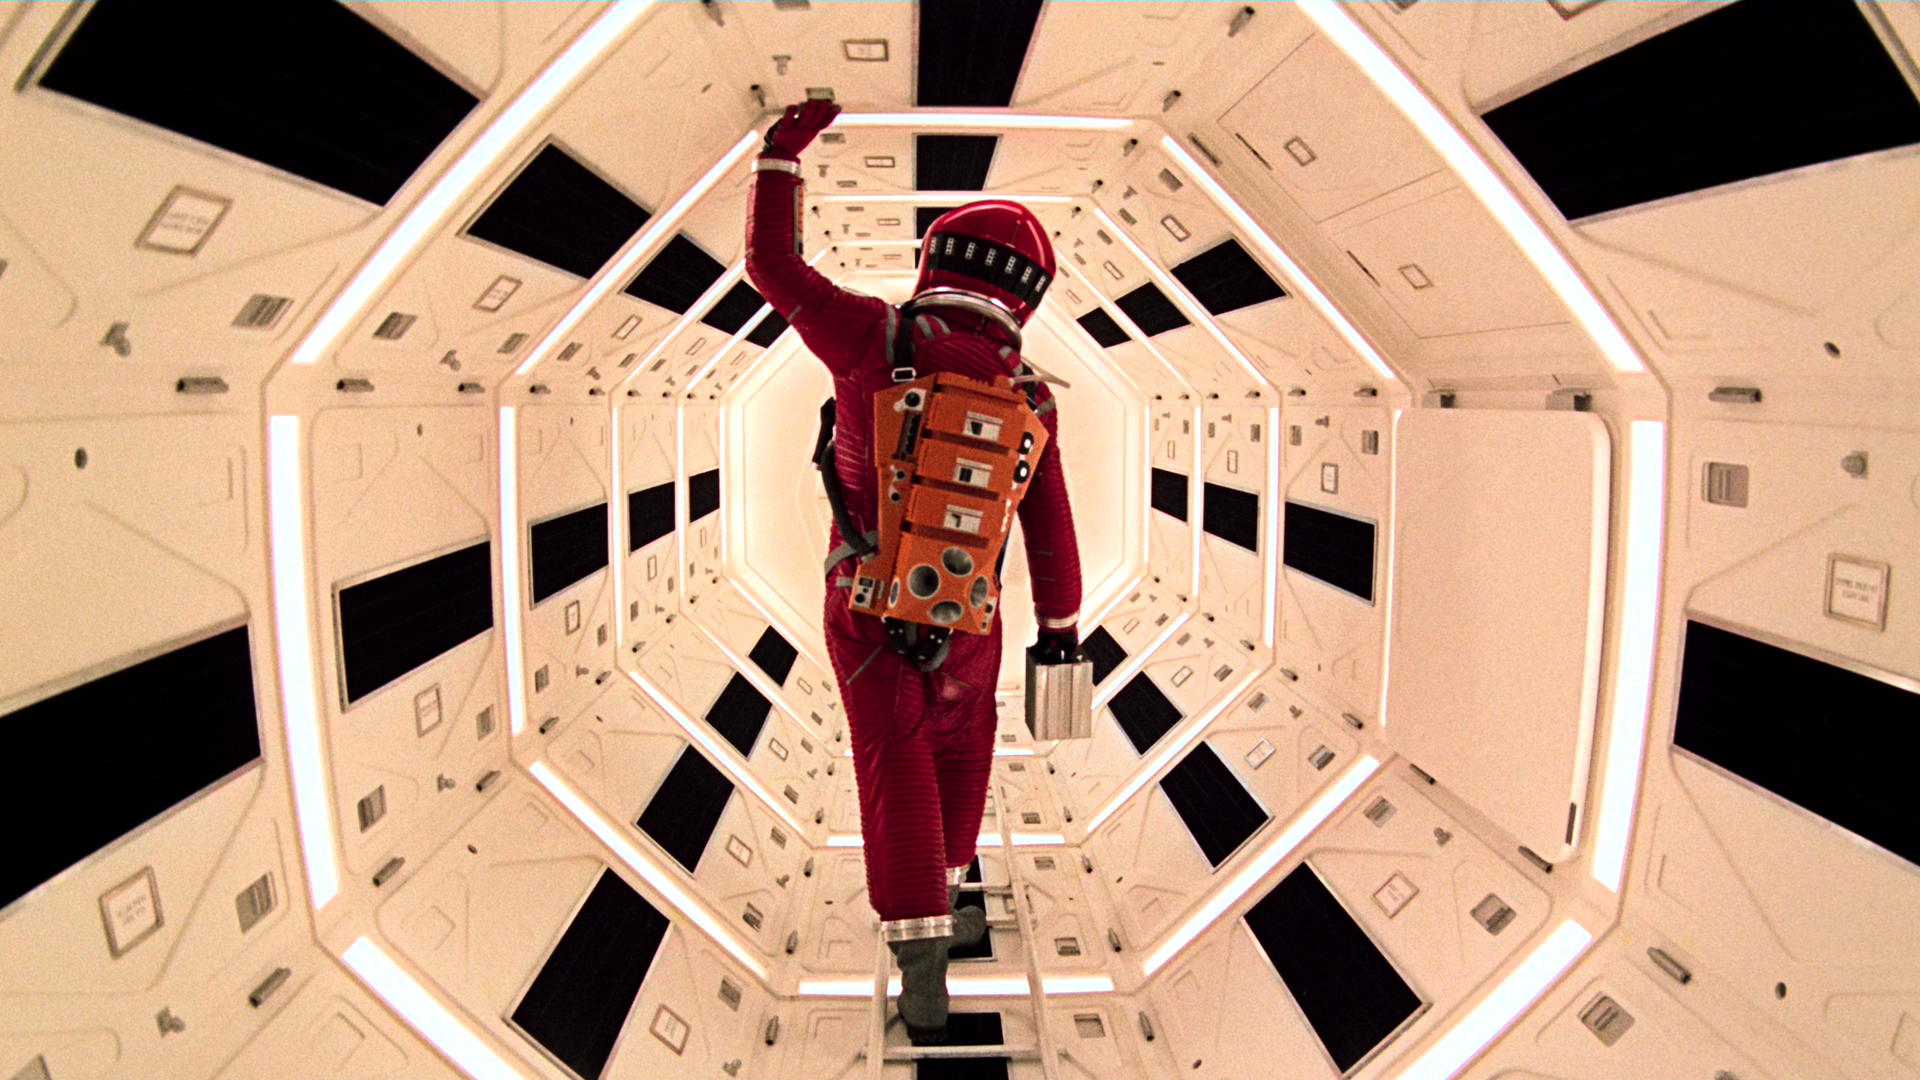
\includegraphics[width=\linewidth]{slike/odiseja.png} % Promenite ime slike i putanju
    \caption{Научна фантастика}
    \label{fig:slika7}
  \end{subfigure}
  \hfill
  \begin{subfigure}{0.45\textwidth}
    \centering
    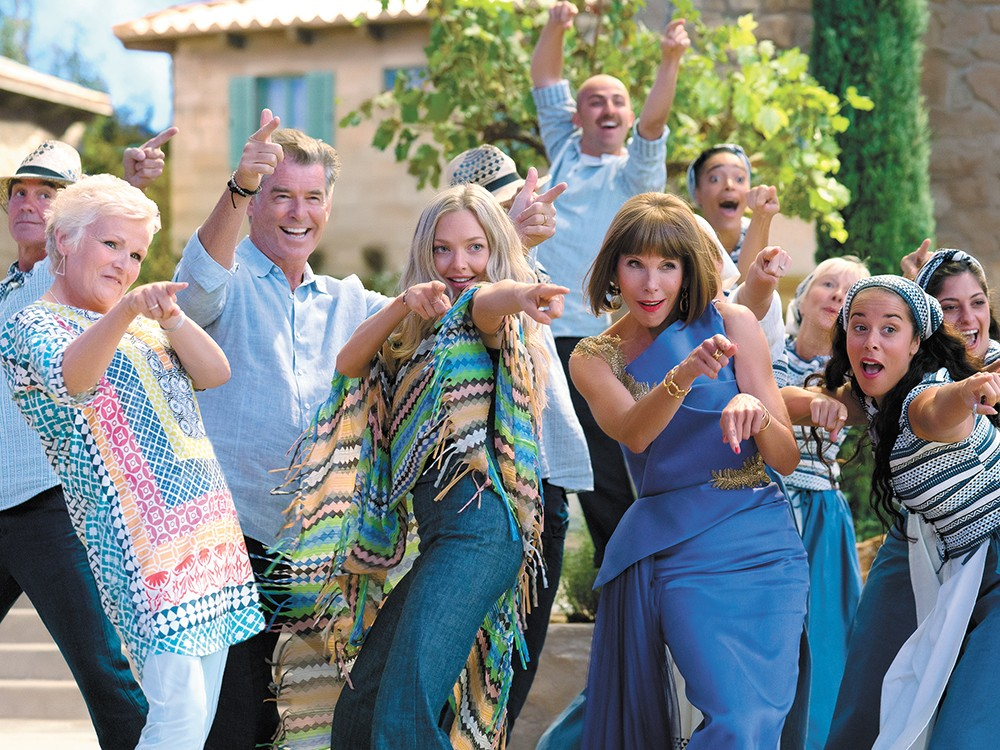
\includegraphics[width=\linewidth]{slike/musical.jpg} % Promenite ime slike i putanju
    \caption{Мјузикл}
    \label{fig:slika8}
  \end{subfigure}
  \caption{жанрови}
  \label{fig:zajednicki_naslov3}
\end{figure}

\begin{figure}[htbp]
  \centering
  \begin{subfigure}{0.45\textwidth}
    \centering
    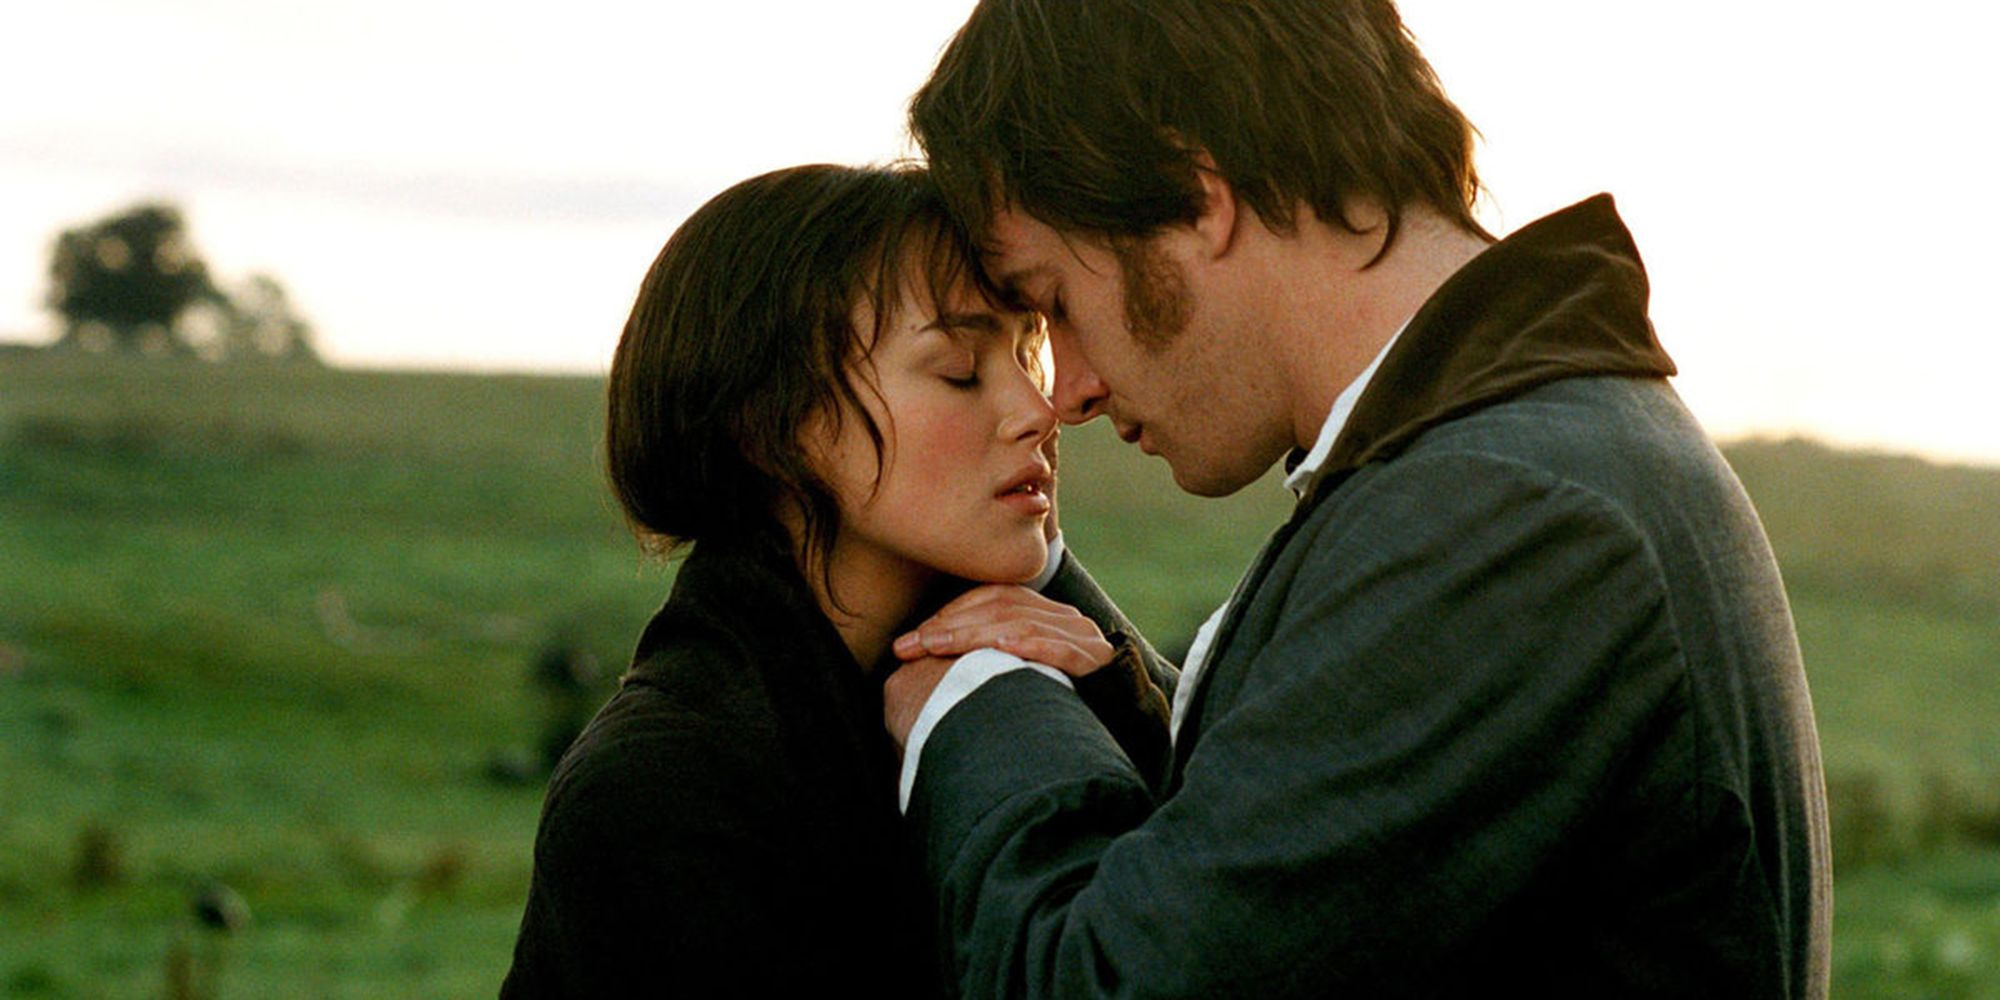
\includegraphics[width=\linewidth]{slike/romantic.jpg} % Promenite ime slike i putanju
    \caption{Романтика}
    \label{fig:slika9}
  \end{subfigure}
  \hfill
  \begin{subfigure}{0.45\textwidth}
    \centering
    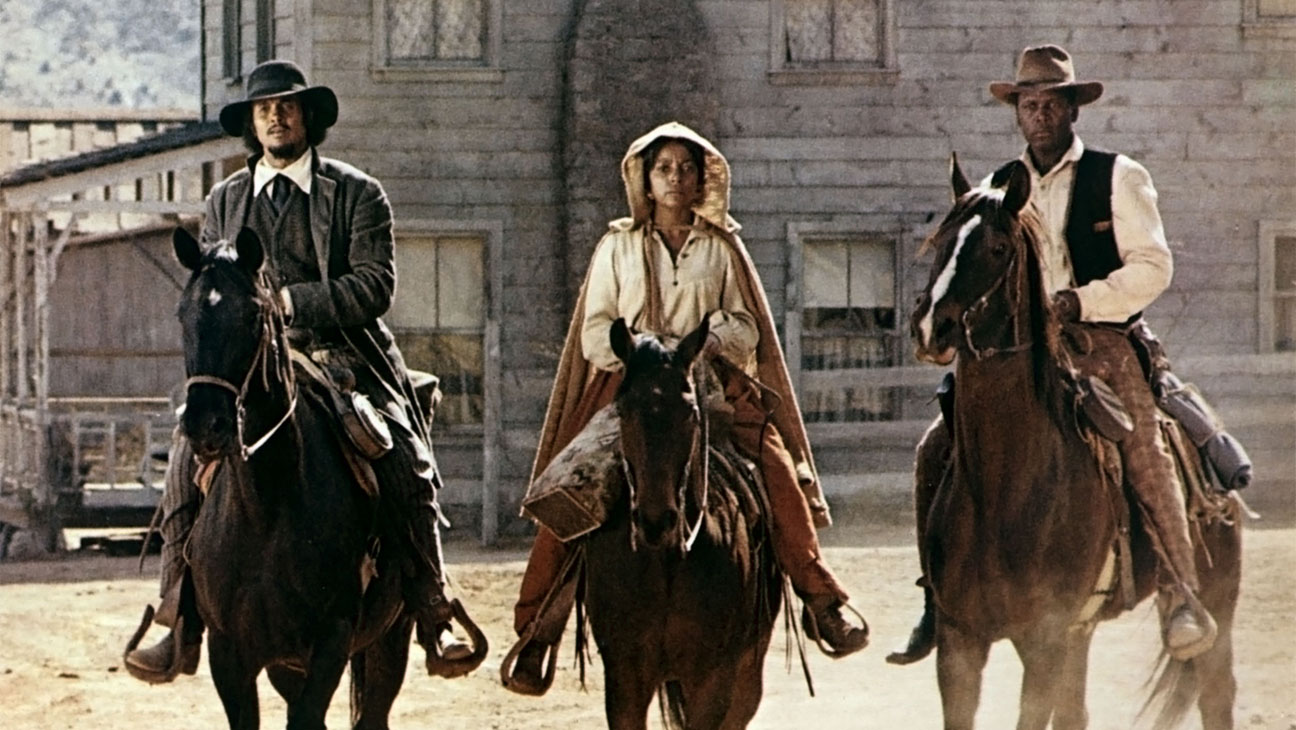
\includegraphics[width=\linewidth]{slike/western.jpg} % Promenite ime slike i putanju
    \caption{Вестерн}
    \label{fig:slika10}
  \end{subfigure}
  \caption{жанрови}
  \label{fig:zajednicki_naslov6}
\end{figure}

\begin{figure}[htbp]
  \centering
  \begin{subfigure}{0.45\textwidth}
    \centering
    
\includegraphics[width=\linewidth]{slike/horor.jpg} % Promenite ime slike i putanju
    \caption{}
    \label{fig:slika9}
  \end{subfigure}
  \hfill
  \begin{subfigure}{0.45\textwidth}
    \centering
    
\includegraphics[width=\linewidth]{slike/horror.png} % Promenite ime slike i putanju
    \caption{}
    \label{fig:slika10}
  \end{subfigure}
  \caption{Хорор}
  \label{fig:zajednicki_naslov6}
\end{figure}

\newpage
\subsection{Класификација и Неуронске Мреже}

Задатак класификације подразумева креирање функције (класификационог модела) која мапира улазне атрибуте $X = (x_1, x_2, \ldots, x_k)$ на једну од предефинисаних вредности $y$, где представља ознаку класе. Циљ модела је да се примени на податке где вредност атрибута $y$ није позната, како би се та вредност што прецизније предвидела.  \\ \\

Обично се улазни подаци деле на два дисјунктна скупа:

\begin{itemize}

\item Скуп за обуку - користи се за креирање модела.
\item Скуп за тестирање - користи се за проверу исправности модела.

\end{itemize}

Такође, могуће је увести и трећи скуп, скуп за валидацију, који се користи током процеса креирања модела како би се спречило претерано прилагођавање модела подацима.  \\ \\


\subsection{Неуронске мреже}
Неуронске мреже тренутно представљају метод машинског учења са најширим
спектром примена. Постоје различите врсте неуронских мрежа, које су често специјализоване за конкретне примене. Датирају из 50-их година двадесетог века и више пута
су у својој историји биле у првом плану истраживања, а потом потиснуте од
стране других метода. 

Свака мрежа састоји се од одређеног броја елементарних јединица које називамо неуронима. Неурони, по грубој аналогији са биолошким неуронима у мозгу, једни
другима прослеђују сигнале и израчунавају нове сигнале на основу оних који су
им прослеђени. Тачна структура повезаности неурона и начин на који они врше
израчунавања чине такозвану архитектуру мреже и прецизно одређују о каквој
мрежи се ради. Архитектуру мреже дефинише експерт, имајући у виду специфичности
проблема који се решава. \\ \\


\subsection{Конволутивне Неуронске Мреже (CNN)}
Захвалјујући конволутивним неуронским мрежама, остварени су највећи помаци у практичним применама машинског учења, пре свега у области рачунарског
вида.
 Разматрамо најпре мотивацију за њихово увођење.
Машинско учење може се користити над сликама за разноврсне задатке, на
пример, за одређивање да ли се на слици налази зграда, да ли се налази семафор, да
ли је на слици мачка или пас, да ли је слика исправно оријентисана, итд. Један приступ
за решавање таквих проблема може бити да се најпре примене вешто осмишљене
трансформације које од слике производе нову слику истих или сличних димензија. Те
трансформације могу бити фокусиране на различите аспекте слике и могу служити да се
слика или њен део изоштри, затамни, да јој се повећа контраст, да се истакну ивице,
итд. Излази таквих трансформација – неке нове слике – онда могу да се користе
као својства на основу којих би модел (попут логистичке регресије или потпуно
повезане мреже) могао да учи.


\section{Имплементација}
У наредним секцијама ћемо детаљније истражити процес креирања личног датасета за анализу спектрограма музике из филмова. Након тога, истражићемо како је овај датасет искоришћен за тренирање конволутивне неуронске мреже. Прво, разматраћемо методологију прикупљања и организације података, а затим ћемо се фокусирати на имплементацију неуронске мреже и анализу резултата. Овај процес представља кључни корак у нашем истраживању и омогућава нам да дубље разумемо звук музике и његову повезаност са жанровима филмова.

\subsection{Прикупљање Података}
Након детаљног истраживања емоционалних карактеристика музике у филмским жанровима, издвојила сам по 50 песама за сваки од наведених жанрова. Одабир песама вршен је пажљиво, како би се осигурало да свака песма јасно репрезентује специфичности свог жанра. Такође, обратила сам посебну пажњу да песме буду довољно различите како би омогућиле прецизну класификацију и како би се избегле евентуалне конфузије међу оцењивачима.

Након што су песме идентификоване и одабране, прешла сам на њихову обраду. Оригинални mp4 фајлови песама конвертовани су у формат .wav, како бих омогућила далу анализу и обраду података. Овај формат је одабран због његове шире употребе и боље подршке за анализу звука и генерисање спектрограма.

Ова пажљиво изведена фаза прикупљања и припреме података била је кључна за бољу анализу и тренирање модела за класификацију филмских жанрова на основу музике. Посвећеност избору и припреми података допринела је поверљивости резултата и омогућила дубље разумевање карактеристика музике у различитим жанровима филма.

\subsection{Прављење Спектрограма}
\textbf{Спектрограм:} Визуелна репрезентација аудио сигнала која приказује фреквенцијски домен сигнала у зависности од времена. Користи се за анализу и обраду аудио података.

За креирање спектрограма користимо библиотеку Librosa у програмском језику Python. Прво, учитавамо аудио фајл у облику низа података:


\begin{verbatim}
import librosa

# Учитавање аудио фајла
audio_signal, sample_rate = librosa.load('audio.wav') 
\end{verbatim}


Након тога, примењујемо трансформацију над аудио сигналом како бисмо креирали спектрограм:

\begin{verbatim}

# Креирање спектрограма
spectrogram = librosa.feature.melspectrogram(y=audio_signal, sr=sample_rate)


\end{verbatim}


Овај процес нам омогућава да визуелно представимо аудио сигнал и анализирамо његове фреквенцијске компоненте у зависности од времена. \\ \\

\begin{figure}[htbp]
  \centering
  \begin{subfigure}{0.45\textwidth}
    \centering
    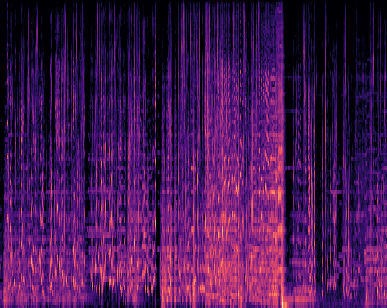
\includegraphics[width=\linewidth]{slike/musical23.png} % Promenite ime slike i putanju
    \caption{Мјузикл}
    \label{fig:slika7}
  \end{subfigure}
  \hfill
  \begin{subfigure}{0.45\textwidth}
    \centering
    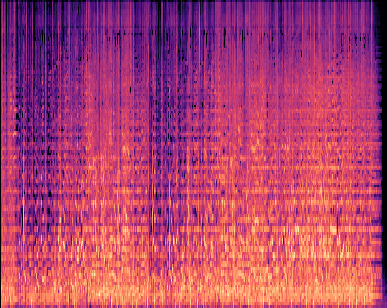
\includegraphics[width=\linewidth]{slike/romantic00.png} % Promenite ime slike i putanju
    \caption{Романтика}
    \label{fig:slika8}
  \end{subfigure}
  \caption{жанрови}
  \label{fig:zajednicki_naslov3}
\end{figure}

\begin{figure}[htbp]
  \centering
  \begin{subfigure}{0.45\textwidth}
    \centering
    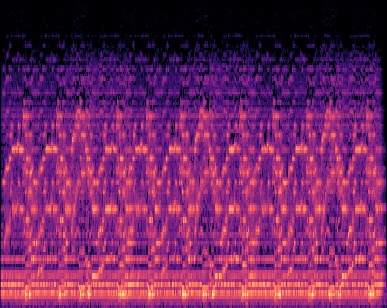
\includegraphics[width=\linewidth]{slike/scifi48.png} % Promenite ime slike i putanju
    \caption{Научна фантастика}
    \label{fig:slika9}
  \end{subfigure}
  \hfill
  \begin{subfigure}{0.45\textwidth}
    \centering
    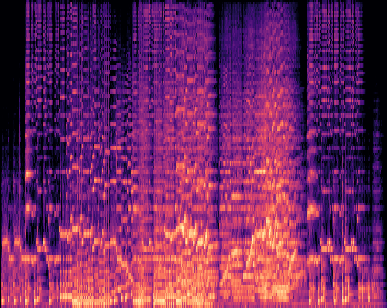
\includegraphics[width=\linewidth]{slike/western06.png} % Promenite ime slike i putanju
    \caption{Вестерн}
    \label{fig:slika10}
  \end{subfigure}
  \caption{жанрови}
  \label{fig:zajednicki_naslov6}
\end{figure}

\begin{figure}[htbp]
  \centering
  \begin{subfigure}{0.45\textwidth}
    \centering
    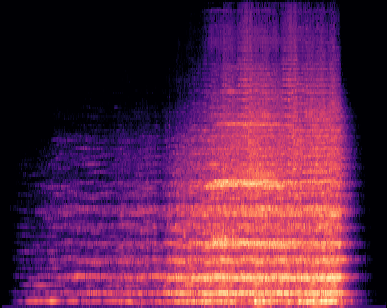
\includegraphics[width=\linewidth]{slike/horror30.png} % Promenite ime slike i putanju
    \caption{}
    \label{fig:slika9}
  \end{subfigure}
  \hfill
  \begin{subfigure}{0.45\textwidth}
    \centering
    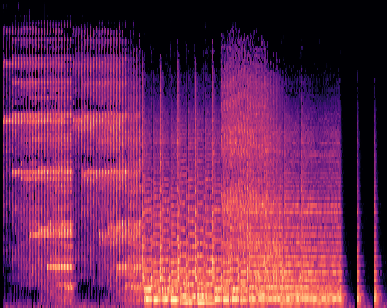
\includegraphics[width=\linewidth]{slike/horror31.png} % Promenite ime slike i putanju
    \caption{}
    \label{fig:slika10}
  \end{subfigure}
  \caption{Хорор}
  \label{fig:zajednicki_naslov6}
\end{figure}

\newpage
\subsection{Креирање Неуронске Мреже}



За први модел (Модел 1), коришћена је  конволутивна неуронска мрежа (CNN) са три слоја конволутивних и три слоја МаксПулинг слојева. Сваки конволутивни слој користи РеЛУ (Ректификована Линеарна Активација) активацију како би се издвојиле одређене карактеристике из спектрограма. Коришћен је и слој за искључивање (Дропаут) са стопом од 0.2 како би се избегло преприлагођавање . На крају, додата су два потпуно повезана (Денсе) слоја за класификацију, са последњим слојем који користи софтмакс активацију како би се добиле вероватноће за сваку класу. \\

Други модел (Модел 2) је веома сличан првом моделу, али је направљен са већим сликама спектрограма како би се ухватило више детаља. Опет је коришћена иста архитектура са три конволутивна слоја, три МаксПулинг слоја, слојем за искључивање (Дропаут), и два потпуно повезана слоја. \\

Трећи модел (Модел 3) користи пренаучену архитектуру ВГГНет са четири конволутивна слоја и два МаксПулинг слоја. Након ВГГНет дела, додата су још три конволутивна слоја, слој за искључивање (Дропаут) и три потпуно повезана слоја за класификацију. Овај модел користи слојеве конволутивне неуронске мреже са већим капацитетом у односу на прва два модела, што омогућава да научи дубље карактеристике из спектрограма. \\

Прва два модела се разликују у резолуцији спектрограма које користе, док трећи модел користи пренаучену архитектуру ВГГНет како би искористио већ научене параметре из других сличних проблема.  \\




\section{Резултати}
Резултати 3 модела која су направљена за класификацију филмских жанрова у односу на музику из филма



\begin{figure}[htbp]
  \centering
  \begin{subfigure}{0.45\textwidth}
    \centering
    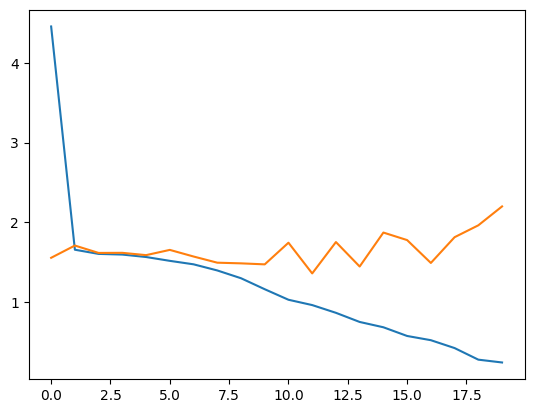
\includegraphics[width=\linewidth]{slike/1loss.png} % Promenite ime slike i putanju
    \caption{Губитак}
    \label{fig:slika1}
  \end{subfigure}
  \hfill
  \begin{subfigure}{0.45\textwidth}
    \centering
    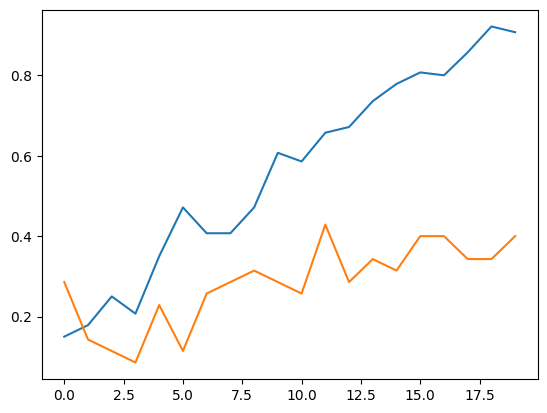
\includegraphics[width=\linewidth]{slike/1acc.png} % Promenite ime slike i putanju
    \caption{Тачност}
    \label{fig:slika2}
  \end{subfigure}
  \caption{Модел 1}
  \label{fig:zajednicki_naslov}
\end{figure}

\begin{figure}[htbp]
  \centering
  \begin{subfigure}{0.45\textwidth}
    \centering
    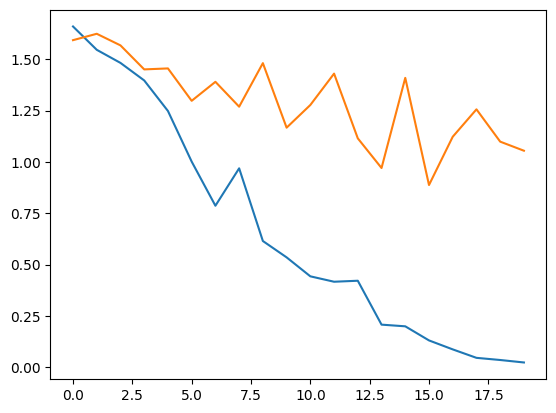
\includegraphics[width=\linewidth]{slike/2loss.png} % Promenite ime slike i putanju
    \caption{Губитак}
    \label{fig:slika3}
  \end{subfigure}
  \hfill
  \begin{subfigure}{0.45\textwidth}
    \centering
    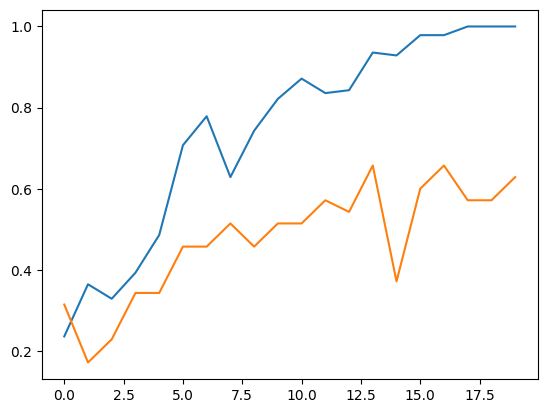
\includegraphics[width=\linewidth]{slike/2acc.png} % Promenite ime slike i putanju
    \caption{Тачност}
    \label{fig:slika4}
  \end{subfigure}
  \caption{Модел 2}
  \label{fig:zajednicki_naslov1}
\end{figure}

\begin{figure}[htbp]
  \centering
  \begin{subfigure}{0.45\textwidth}
    \centering
    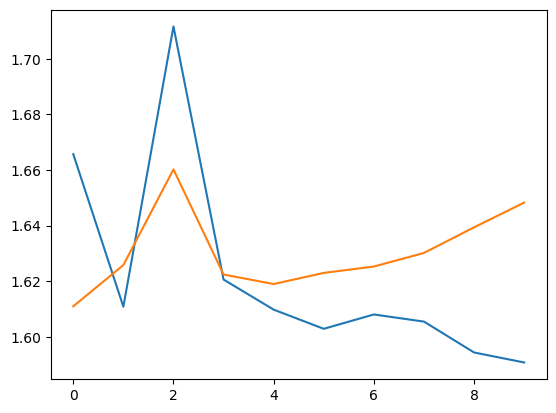
\includegraphics[width=\linewidth]{slike/3loss.png} % Promenite ime slike i putanju
    \caption{Губитак}
    \label{fig:slika5}
  \end{subfigure}
  \hfill
  \begin{subfigure}{0.45\textwidth}
    \centering
    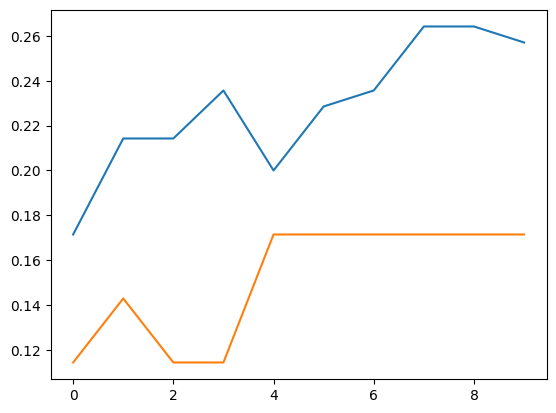
\includegraphics[width=\linewidth]{slike/3acc.png} % Promenite ime slike i putanju
    \caption{Тачност}
    \label{fig:slika6}
  \end{subfigure}
  \caption{Модел 3}
  \label{fig:zajednicki_naslov}
\end{figure}


У  пројекту  је коришћено ограничен број података за обуку модела. Интересантно је приметити да су прва два модела показала значајно боље перформансе у поређењу са трећим моделом који користи пренаучену архитектуру.

Разлог зашто је трећи модел био мање ефикасан може се објаснити на следећи начин:

1. \textbf{Недостатак прилагођавања подацима}: Пренаучени модели често захтевају фино подешавање параметара како би се прилагодили специфичним подацима. У нашем случају, можда је било потребно пажљиво прилагодити трећи модел нашим ограниченим подацима, што није адекватно урађено.

2. \textbf{Велика сложеност архитектуре}: Пренаучене архитектуре могу бити веома сложене и захтевати велики број параметара. Ако имамо мало података, може доћи до проблема са преприлагођавањем (overfitting), где модел научи податке за обуку "напамет" уместо да генерализује на нове податке.

3. \textbf{Недостатак доступних података за фино подешавање}: За фино подешавање пренаучених модела често су потребни додатни подаци који су слични онима на којима је модел првобитно трениран. Ако такви подаци нису доступни, може бити тешко постићи добре резултате са пренаученим моделима.

Како бисмо побољшали перформансе трећег модела, можемо разматрати додавање више података за обуку, фино подешавање параметара или разматрање мање сложених пренаучених архитектура које боље одговарају нашим ограничењима.
Такође због специфичности пројекта више су упоређивани модели у пројекту него са другим пројектима јер не постоје на ту тему.

\section{Закључак}
Циљ пројекта био је истраживање и развој модела за класификацију филмских жанрова на основу карактеристика музике из филмова. Музика има значајан утицај на емотивну перцепцију и атмосферу филма, па је разумевање како се ове карактеристике препознају и класификују могу бити од  значаја. Прикупљање података за ову врсту задатка је изазовно, али од кључне важности. Пажљиво је креиран датасет од 250 песама, са по 50 песама за сваки од пет анализираних жанрова. Овај датасет је био основа за обуку и тестирање модела.  За обраду спектрограма музике, коришћена је  конволутивна неуронска мрежа (CNN). Развијена су три различита модела са различитим архитектурама како би се истражила ефикасност у класификацији жанрова.

\section{Референце}
[1] P. Janičić, M. Nikolić. \textit{Veštačka inteligencija}. Matematički fakultet, 2021.
\indent[2] Librosa : https://librosa.org/doc/latest/index.html


\end{document}
